\documentclass[
    10pt,
    aspectratio=169,
    xcolor={dvipsnames},
    spanish,
    % handout,
    % notes=only,
    % notes,
    ]{beamer}

% BEAMER SETTINGS
\setbeamerfont{section in toc}{size=\normalsize, shape=\bfseries}
\mode<presentation>{
    \usetheme{Antibes}
    \setbeamercovered{transparent}
    \usecolortheme{rose}
    \setbeamertemplate{navigation symbols}{}
    }
\useoutertheme{infolines}

% PACKAGES
% \usepackage[spanish]{babel}  % uncomment for Spanish support
\usepackage{tikz,pgfplots}
\pgfplotsset{compat=1.13}
\usetikzlibrary{calc}
\usepackage{subcaption}
\usepackage{graphicx}
\graphicspath{{figures}}
\usepackage{booktabs}
\usepackage{upgreek}
\usepackage{commath}
\usepackage{amsmath,amsthm,amssymb,mathtools,mathrsfs}
\usepackage{cancel}
\usepackage{fontawesome5}
\usepackage{enumerate}
\usepackage{tensor}
\usepackage[font=footnotesize]{caption}
\usepackage{wasysym}

\usepackage[skins,theorems]{tcolorbox}
\tcbset{
    highlight math style={
        enhanced,
        coltext=black,
        colframe=black,
        colback=lightgray,
        arc=0pt,
        boxrule=.5pt
        }
}

% REFERENCES AND OTHERS
\usepackage{aas_macros}
\usepackage{natbib}
\bibpunct{(}{)}{;}{a}{}{,}

\usepackage{siunitx}
\sisetup{
    range-phrase=\text{--},
    range-units=single,
    separate-uncertainty=true,
    print-unity-mantissa=false
    }
\DeclareSIUnit{\gauss}{G}
\DeclareSIUnit{\jansky}{Jy}
\renewcommand{\figurename}{Fig.}

\usepackage{hyperref}
\hypersetup{
    % bookmarks=true,
    unicode=true,
    pdftoolbar=true,
    pdfmenubar=true,
    pdffitwindow=false,
    pdfstartview={FitH},
    pdftitle={ISI-Free Linear Combination Pulses with Better Performanc},
    pdfauthor={Erik Saez A.},
    pdfcreator={Erik Saez A.},
    pdfnewwindow=true,
    colorlinks=true,
    linkcolor=RoyalBlue,
    citecolor=RoyalBlue,
    urlcolor=RoyalBlue
    }

\title[Auxiliar \#1]{\bfseries Auxiliar \#1}
\subtitle{}
\author[Erik Saez A.]{Erik Saez A.}
\institute[UChile]{Department of Electrical Engineering \\ Universidad de Chile}

\date{\today}

\begin{document}

\begin{frame}
  \titlepage
  \centering
  \faIcon{envelope} \href{mailto:erik.saez@ug.uchile.cl}{erik.saez@ug.uchile.cl} \hspace{.2cm}
\end{frame}

\begin{frame}
  \frametitle{Contenidos}
  \centering
  \begin{columns}
    \begin{column}{0.4\textwidth}
      \tableofcontents
    \end{column}
    \begin{column}{0.5\textwidth}
      \begin{figure}
        \centering
        
\includegraphics[width=\textwidth]{fcfm_die}
        \caption{Facultad de Ciencias Físicas y Matemáticas , Universidad de Chile.}
      \end{figure}
    \end{column}
  \end{columns}  
\end{frame}
%%%%%%%%%%%%%%%%%%%%%%%%%%%%%%%%%%%%%%%%%%

\section{Motivación}
\begin{frame}{Motivación}
  \begin{itemize}
    \item ¿Por qué vale la pena tomar este ramo?
    \item ¿Qué me puede aportar si no pienso dedicarme al área de Control?
    \item ¿Es realmente importante ir a clases? 
    \item ¿Qué cosas interesantes voy a aprender aquí?
    \item \dots
  \end{itemize}
\end{frame}
%%%%%%%%%%%%%%%%%%%%%%%%%%  
\section{Aspectos Generales del curso}


%%%%%%%%%%%%%%%%%%%%%%%%%%%
\begin{frame}{Continuidad del ramo}
  \begin{itemize}
    \item Análisis de sistemas dinámicos $\rightarrow$ Fundamentos de control de sistemas.
    \item ¡Atrasa! pero no es crítico
  \end{itemize}
  \begin{figure}
    \centering
    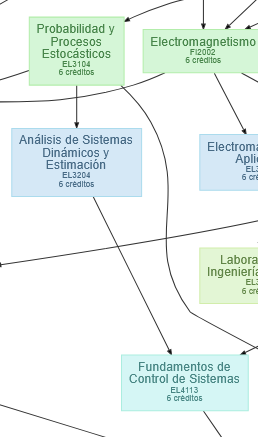
\includegraphics[width=0.2\textwidth]{Figura_1.png}
    \caption{Continuidad del ramo}
  \end{figure}
\end{frame}
%%%%%%%%%%%%%%%%%%%%%%%%%
\begin{frame}{Evaluaciones del ramo}
\begin{columns}
  \begin{column}{0.55\textwidth}
    \begin{block}{Tipos de Evaluación}
      \begin{table}[h]
        \centering
        \footnotesize
        \begin{tabular}{|l|l|}
        \hline
        \textbf{Tipo} & \textbf{Descripción} \\
        \hline
        Controles (2) & Control 1 y Control 2 \\
        \hline
        Ejercicios (2) & Ejercicio 1 y Ejercicio 2 \\
        \hline
        Proyecto & Unidades 2 y 3 \\
        \hline
        Examen & Toda la materia \\
        \hline
        \end{tabular}
      \end{table}
      
      \vspace{0.2cm}
      \textbf{Cálculo de Nota Final:}
      \begin{itemize}
        \item \textbf{NF = NC × 0.6 + NE × 0.4}
        \item \textbf{NC}: Controles (incluye Examen 50\%)
        \item \textbf{NE}: Promedio Ejercicios
      \end{itemize}
    \end{block}
  \end{column}
  
  \begin{column}{0.43\textwidth}
    \begin{alertblock}{Recomendaciones}
      \scriptsize
      \begin{itemize}
        \item Control 1: bastante materia, suele ser complejo
        \item Ejercicios son largos, no dejar para último momento
        \item Consulten dudas las veces que sea necesario
      \end{itemize}
    \end{alertblock}
  \end{column}
\end{columns}
\end{frame}
%%%%%%%%%%%%%%%%%%%%%%%%

\section{Resumen de Conceptos}

\begin{frame}{Importancia de las Hipótesis Simplificatorias}
\begin{block}{¿Por qué son importantes las hipótesis?}
  \begin{itemize}
    \item \textbf{Simplifican el modelo}: Permiten obtener ecuaciones manejables
    \item \textbf{Definen el alcance}: Establecen bajo qué condiciones es válido el modelo
    \item \textbf{Balance realismo-simplicidad}: Mantienen las características esenciales del sistema
    \item \textbf{Facilitan el análisis}: Hacen posible aplicar herramientas matemáticas conocidas
  \end{itemize}
\end{block}

\begin{alertblock}{Advertencia}
  \begin{itemize}
    \item Hipótesis muy restrictivas $\rightarrow$ Modelo poco realista
    \item Hipótesis muy generales $\rightarrow$ Modelo muy complejo
    \item \textbf{Clave}: Encontrar el balance adecuado para cada problema
  \end{itemize}
\end{alertblock}
\end{frame}

%%%%%%%%%%%%%%%%%%%%%%%%
%%%%%%%%%%%%%%%%%%%%%%%%
\begin{frame}{Estados Especiales de un Sistema}
\begin{columns}
  \begin{column}{0.48\textwidth}
    \begin{block}{Estado Cero}
      \footnotesize
      Un estado cero $x_0 \in \Sigma$ de un sistema es tal que la salida $y(t)$ cumple que:
      \begin{equation}
        y(t) = \overline{A}(x_0, 0) = 0. \tag{1}
      \end{equation}
      \textbf{En términos sencillos}: Es una condición inicial tal que, para entrada cero, la salida es cero.
    \end{block}
    
    \begin{block}{Estado Tierra}
      \footnotesize
      Un estado tierra $x_t \in \Sigma$ de un sistema es tal que:
      \begin{equation}
        \forall x_0 \in \Sigma, \lim_{t \to \infty} \overline{B}(x_0, 0) = x_t. \tag{2}
      \end{equation}
      \textbf{Significado}: El estado tierra es tal que, para toda condición inicial y con entrada cero, el sistema converge al estado tierra.
    \end{block}
  \end{column}
  
  \begin{column}{0.48\textwidth}
    \footnotesize
    \begin{block}{Estado Equilibrio}
      Un estado equilibrio $x_e \in \Sigma$ es tal que:
      \begin{equation}
        x_e = \overline{B}(x_e, 0). \tag{3}
      \end{equation}
      \textbf{Significado}: Bajo entrada cero, si el sistema está en estado equilibrio entonces se quedará por siempre en este.
    \end{block}
    
    \vspace{0.5cm}
    
    \begin{alertblock}{Nota Importante}
      \scriptsize
      Estos conceptos son fundamentales para el análisis de estabilidad y diseño de controladores en sistemas dinámicos.
    \end{alertblock}
  \end{column}
\end{columns}
\end{frame}

%%%%%%%%%%%%%%%%%%%%%%%%
\begin{frame}{Linealización de Sistemas}
\begin{columns}
  \begin{column}{0.48\textwidth}
    \begin{block}{Linealización}
      \scriptsize
      Sistema dinámico:
      \begin{align}
        \dot{x} &= f(x, u) \\
        y &= g(x, u)
      \end{align}
      
      Sistema linealizado en $\overline{x}, \overline{u}$:
      \begin{align}
        \dot{\tilde{x}} &= \frac{\partial f}{\partial x}\bigg|_{\overline{x},\overline{u}} \tilde{x} + \frac{\partial f}{\partial u}\bigg|_{\overline{x},\overline{u}} \tilde{u} \\
        \tilde{y} &= \frac{\partial g}{\partial x}\bigg|_{\overline{x},\overline{u}} \tilde{x} + \frac{\partial g}{\partial u}\bigg|_{\overline{x},\overline{u}} \tilde{u}
      \end{align}
    \end{block}
  \end{column}
  
  \begin{column}{0.48\textwidth}
    \begin{block}{Variables Perturbadas}
      \scriptsize
      Las variables perturbadas se definen como:
      \begin{align}
        \tilde{x} &\triangleq x - \overline{x} \\
        \tilde{u} &\triangleq u - \overline{u} \\
        \tilde{y} &\triangleq y - \overline{y}
      \end{align}
      
      donde $\tilde{x}, \tilde{u}, \tilde{y}$ representan las perturbaciones en torno al estado, entrada y salida de operación, respectivamente.
    \end{block}
  \end{column}
\end{columns}
\end{frame}



%%%%%%%%%%%%%%%%%%%%%%%%
\section{Pregunta 1}
\begin{frame}{Pregunta \#1}
\begin{block}{Enunciado Pregunta \#1}
  \footnotesize
   Considere el sistema de la siguiente figura, donde se tiene un carro atado a un resorte con un sensor de distancia, capaz de medir la distancia del carro a la pared. Suponga que existe una fuerza de fricción viscosa con la superficie $F_f$ de la forma $F_f = b_1 \dot{z} + b_2 (\dot{z}^2)$.
    \begin{figure}[ht]
        \centering
        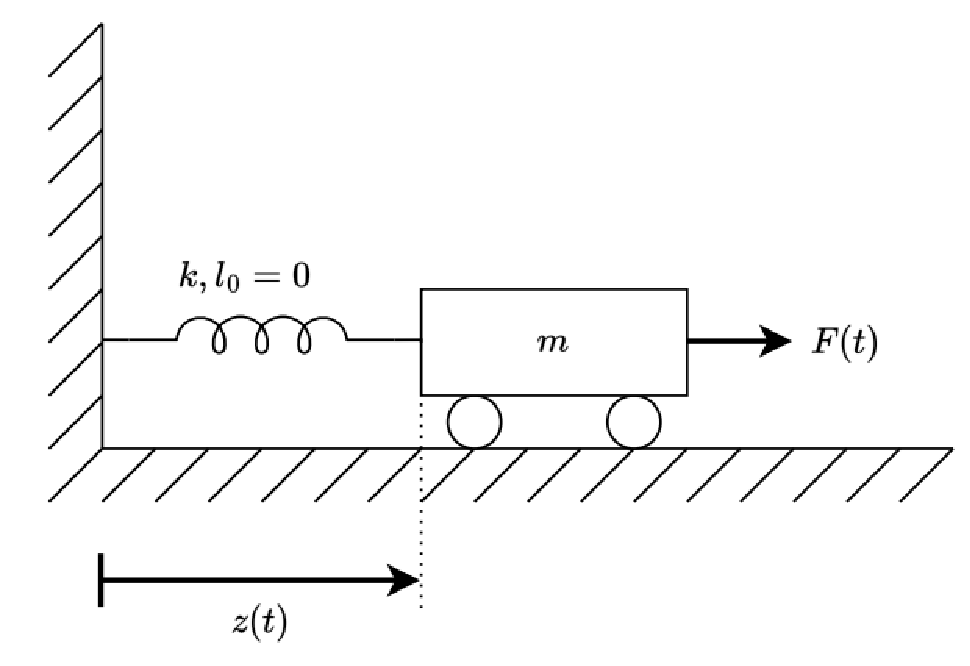
\includegraphics[width=0.3\textwidth]{Figura_2.pdf}
    \end{figure}
    \begin{enumerate}
        \item Establezca hipótesis simplificatorias para el problema.
        \item Formule un modelo matemático del sistema que sea consistente con sus hipótesis.
        \item Encuentre el punto de operación que asegure $z = 1$ m.
    \end{enumerate}
\end{block}
\end{frame}
%%%%%%%%%%%%%%%%%%%%%%
\section{Pregunta 2}
\begin{frame}{Pregunta \#2}
  \begin{block}{Enunciado Pregunta \#2}
  Considere el siguiente péndulo apoyado en un carro móvil, el cual se desliza por una barra.
    \begin{enumerate}
        \item Establezca hipótesis simplificatorias.
        \item Formule un modelo matemático, que capture la dinámica del sistema.
        \item Identifique entradas, salidas y estados en su modelo.
        \item Linealice en torno a $\theta = \pi$.
    \end{enumerate}
    \begin{figure}[ht]
        \centering
        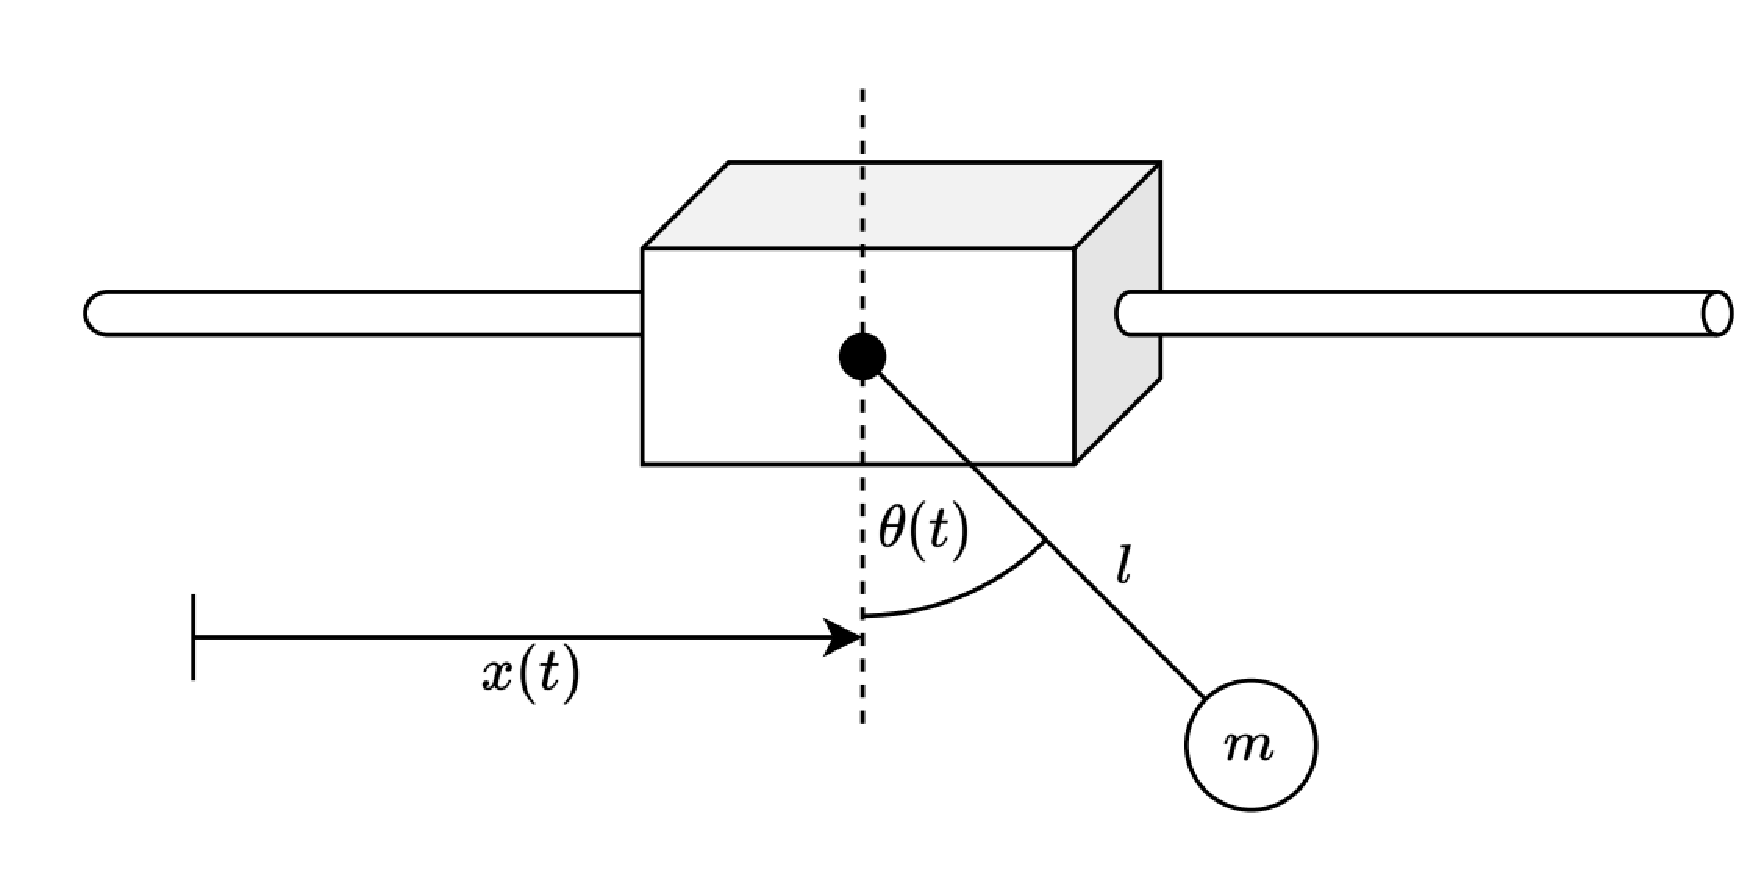
\includegraphics[width=0.4\textwidth]{Figura_3.pdf}
    \end{figure}
  \end{block}
\end{frame}

%%%%%%%%%%%%%%%%%%%%%%
\section{Pregunta 3}
\begin{frame}{Pregunta \#3: Estanque Cónico}
\vspace{-0.35cm}
\begin{columns}
    % Columna izquierda con figura y datos
    \begin{column}{0.34\textwidth}
      \vspace{-0.2cm}
      \begin{figure}[ht]
          \centering
          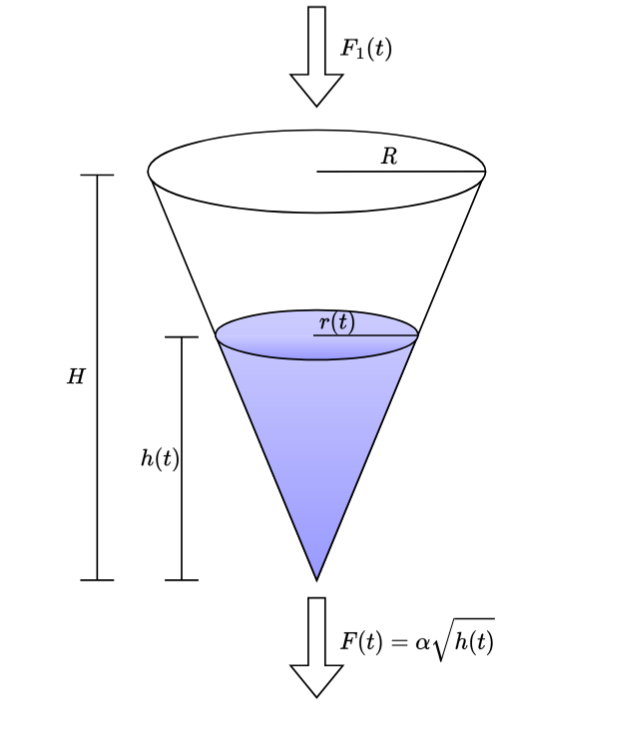
\includegraphics[width=0.63\textwidth]{Figura_4.png} % más pequeña
      \end{figure}
      \scriptsize
      \begin{block}{Datos del Sistema}
        \setlength\itemsep{0.1em}
        \begin{itemize}
            \item Altura máxima: $H = 8$ m
            \item Radio máximo: $R = 3$ m
            \item Volumen: $V(h) = \frac{\pi r^2 h}{3}$
            \item Flujo entrada: $F_1(t)$ (arbitrario)
            \item Flujo salida: $F(t) = \alpha \sqrt{h(t)}$, $\alpha = 1$
        \end{itemize}
      \end{block}
    \end{column}
    
    % Columna derecha con enunciado completo
    \begin{column}{0.64\textwidth}
      \scriptsize
      \begin{block}{Enunciado}
        Se tienen los siguientes datos y relaciones para el estanque cónico:
        \[
        V(h) = \frac{\pi r^2 h}{3}, \quad
        F(t) = \alpha \sqrt{h(t)}, \quad \alpha = 1
        \]
        \textbf{Responda lo siguiente:}
        \begin{enumerate}
            \setlength\itemsep{0.2em}
            \item Encuentre un modelo dinámico no lineal que relacione $h(t)$ y $F_1(t)$, indicando claramente las hipótesis simplificatorias.
            \item Linealice su modelo en torno a $h_0 = 4$ m, $F_{1,0} = 2$ m³/s, para el modelo perturbado:
            \[
                h(t) = h_0 + \Delta h(t), \quad 
                F_1(t) = F_{1,0} + \Delta F_1(t)
            \]
            que relacione la salida $\Delta h(t)$ con la entrada $\Delta F_1(t)$, despreciando términos de orden superior.
        \end{enumerate}
      \end{block}
    \end{column}
  \end{columns}
\end{frame}

\end{document}
